\chapter{Cơ sở lý thuyết và nghiên cứu liên quan}
\label{chap:background}

\section{MCI và tiến triển Alzheimer}
MCI mô tả suy giảm nhận thức vượt mức kỳ vọng theo tuổi nhưng chưa làm mất tính độc lập như sa sút trí tuệ. Đây là trạng thái không đồng nhất về nguyên nhân và diễn biến; chỉ một phần người bệnh tiến triển sang AD \cite{petersen2018mci}. Khái niệm lâm sàng này cũng cần được phân biệt với định nghĩa AD theo các dấu ấn sinh học trong khung nghiên cứu NIA-AA \cite{jack2018niaaa}. Khóa luận dùng nhãn tiến triển vận hành của project, không coi điểm nguy cơ do mạng sinh ra là bằng chứng xác nhận bệnh lý AD.

Trong nghiên cứu tiên lượng, câu hỏi là một sự kiện sẽ được ghi nhận khi nào sau giai đoạn quan sát. Ba visit có thể cho biết cùng một đặc điểm não đang ổn định hay thay đổi; MRI, radiomics và lâm sàng cung cấp những góc nhìn khác nhau về quá trình đó. Cơ sở dữ liệu ADNI hỗ trợ khảo sát các tín hiệu hình ảnh, lâm sàng và nhận thức theo thời gian \cite{weiner2015impact}. Tuy nhiên, điều kiện phải có đủ chuỗi visit cũng làm cohort nghiên cứu khác với toàn bộ người MCI, đặc biệt với những người tiến triển sớm hoặc thiếu theo dõi.

\section{Mô hình dọc và phân tích sống còn}
\subsection{Sự kiện, kiểm duyệt và mô hình Cox}
Gọi $T_i$ là thời gian quan sát và $\delta_i\in\{0,1\}$ là chỉ báo sự kiện. Với kiểm duyệt phải, $\delta_i=0$ chỉ cho biết chưa quan sát sự kiện đến thời điểm kết thúc theo dõi. Phân tích sống còn giữ lại thông tin thời gian và trạng thái kiểm duyệt; phân loại nhị phân tại một cửa sổ cố định trả lời một câu hỏi khác.

Mô hình Cox proportional hazards biểu diễn hazard của bệnh nhân $i$ như sau \cite{cox1972regression}:
\begin{equation}
 h_i(t)=h_0(t)\exp(\eta_i),
\end{equation}
trong đó $h_0(t)$ là baseline hazard và $\eta_i$ là log-risk. DeepSurv là một ví dụ về cách dùng mạng neural để học log-risk phi tuyến trong mô hình Cox \cite{katzman2018deepsurv}. Trong khóa luận, $\eta_i$ được thay bằng đầu ra của survival head. Chỉ số này xếp hạng nguy cơ; để có xác suất tiến triển theo một thời hạn còn cần ước lượng baseline survival và đánh giá calibration.

Với risk set $\mathcal{R}(t_i)$ gồm những người còn được theo dõi tại $t_i$, trường hợp không có ties cho negative partial log-likelihood
\begin{equation}
\mathcal{L}_{\mathrm{Cox}}
=-\sum_{i:\delta_i=1}\left(\eta_i-\log\sum_{j\in\mathcal{R}(t_i)}\exp(\eta_j)\right).
\end{equation}
Các sự kiện trùng thời gian được xử lý bằng xấp xỉ Breslow \cite{breslow1974covariance}; biểu thức nhóm ties của implementation được trình bày ở Chương~\ref{chap:method}. Harrell C-index đo khả năng sắp xếp đúng thứ tự trên các cặp có thể so sánh \cite{harrell1996multivariable}. C-index đánh giá phân biệt, không tự chứng minh calibration hoặc ích lợi lâm sàng; quy tắc xử lý ties cũng cần thống nhất khi so sánh.

Landmarking là cách đặt một mốc thời gian để xét ai còn đủ điều kiện được theo dõi trước khi dự báo kết cục tiếp theo \cite{vanhouwelingen2007dynamic}. Trong khóa luận, $L$ là ngày kết thúc khoảng chọn mẫu, bằng ngày khám ban đầu cộng 18 tháng theo lịch; còn $p$ là ngày MRI thứ ba và là mốc bắt đầu tính thời gian. Chỉ những người chưa chạm ngưỡng tiến triển đến hết $L$ mới được chọn, nên kết quả phản ánh riêng nhóm này. Thông tin lâm sàng ghép trong vòng 90 ngày có thể được ghi sau MRI, vì vậy chưa chắc đã có sẵn tại ngày $p$.

\subsection{T-LSTM và attention theo visit}
Long Short-Term Memory (LSTM) dùng trạng thái bộ nhớ và các gate để tổng hợp thông tin trong chuỗi \cite{hochreiter1997lstm}; khoảng thời gian không đều giữa hai lần khám không tự được mã hóa chỉ bằng thứ tự visit. Time-Aware LSTM (T-LSTM) sử dụng $\Delta t$ để điều chỉnh một thành phần bộ nhớ theo thời gian đã trôi qua \cite{baytas2017patient}. Đây là cơ chế phù hợp với khoảng cách visit không đều; mức lợi ích so với baseline vẫn phải được kiểm tra trên dữ liệu cụ thể.

Attention tổng hợp các hidden state $h_t$ bằng trọng số học được. Khóa luận dùng một phép chấm điểm cộng theo tinh thần additive attention \cite{bahdanau2015attention}:
\begin{equation}
 e_t=\bm v^{\top}\tanh(W_h h_t+b_h),\qquad
 \alpha_t=\frac{\exp(e_t)}{\sum_k\exp(e_k)},\qquad
 z=\sum_t\alpha_t h_t.
\end{equation}
Trọng số $\alpha_t$ mô tả cách mô hình tổng hợp visit trong lần suy luận đó; bản thân chúng không đủ để suy ra tầm quan trọng nhân quả của một lần khám.

\section{Thông tin đa phương thức}
\subsection{MRI cấu trúc và biểu diễn học sâu}
Convolutional Neural Network (CNN) học bộ lọc cục bộ với trọng số dùng chung trên ảnh \cite{lecun1998gradient}. CNN 3D mở rộng phép tích chập sang ba chiều; C3D là một công trình nền tảng cho đặc trưng không gian--thời gian trong video \cite{tran2015c3d}. Với MRI thể tích, cả ba trục đều là trục không gian, còn các visit được xử lý bởi mô hình thời gian riêng. ResNet sử dụng các kết nối residual để học phần hiệu chỉnh trên một nhánh truyền thông tin gốc \cite{he2016deep}. MedicalNet/Med3D cung cấp hướng tiền huấn luyện và transfer learning cho ảnh y tế 3D \cite{chen2019med3d}. Khóa luận khảo sát các baseline MRI trước khi cố định cấu hình encoder cho các so sánh fusion có kiểm soát.

Batch normalization chuẩn hóa theo thống kê mini-batch trong backbone \cite{ioffe2015batchnorm}; layer normalization dùng thống kê trên biểu diễn của từng mẫu và được sử dụng sau hợp nhất \cite{ba2016layernorm}. ReLU \cite{nair2010rectified} và GELU \cite{hendrycks2016gelu} là các hàm kích hoạt được dùng theo từng khối của implementation. Những thành phần này hỗ trợ tối ưu, không phải các đóng góp mới của khóa luận.

\subsection{Vision Transformer và biểu diễn ảnh 3D}
Transformer sử dụng attention để học quan hệ giữa các token \cite{vaswani2017attention}. Vision Transformer (ViT) áp dụng ý tưởng này cho chuỗi patch ảnh \cite{dosovitskiy2021vit}. Khi mở rộng sang thể tích, patch có ba chiều và attention có thể liên kết những vùng xa nhau; UNETR minh họa encoder Transformer cho ảnh y tế 3D trong tác vụ segmentation \cite{hatamizadeh2022unetr}. Đây là nền tảng của hướng ViT 3D, còn khả năng tiên lượng tiến triển cần được đánh giá bằng một protocol riêng.

CrossFormer gốc học cross-scale embeddings và attention ở khoảng cách ngắn/dài trên ảnh 2D \cite{wang2022crossformer}. Các track so sánh trong project dùng bản thích nghi CrossFormer3D Tiny cho MRI thể tích. Tên này được giữ trong phần thực nghiệm để xác định đúng backbone đã khảo sát; các paper ViT và UNETR cung cấp cơ sở lý thuyết, còn encoder của kiến trúc cuối là ResNet-18 3D khởi tạo từ MedicalNet.

\subsection{Radiomics và giảm chiều}
PyRadiomics trích xuất các descriptor định lượng từ ảnh và vùng quan tâm, bao gồm hình dạng, cường độ và kết cấu \cite{vangriethuysen2017computational}. Radiomics và CNN embedding cùng bắt nguồn từ MRI nhưng dùng hai cách biểu diễn khác nhau; vì vậy chúng có thể vừa bổ sung vừa trùng lặp thông tin. Principal Component Analysis (PCA) tạo những hướng tuyến tính trực giao tối đa hóa phương sai và được dùng để giảm chiều đầu vào \cite{jolliffe2016pca}. PCA không tối ưu trực tiếp khả năng tiên lượng; số thành phần và mọi thống kê chuẩn hóa phải được fit từ training split trong quy trình đánh giá.

\subsection{Biến lâm sàng và observedness masks}
Các thước đo như MMSE và CDR cung cấp thông tin về nhận thức và mức suy giảm chức năng \cite{folstein1975mmse,morris1993cdr}. Clinical branch trong project nhận giá trị sau tiền xử lý cùng observedness masks. Mask cho phép mô hình phân biệt một giá trị được quan sát với một giá trị được điền thay thế. Tuy nhiên, mask không khắc phục sai lệch do cơ chế thiếu dữ liệu hoặc việc đo sau thời điểm dự báo; quy tắc căn chỉnh vẫn phải được báo cáo riêng.

\section{Các chiến lược hợp nhất đa phương thức}
Học đa phương thức cần phân biệt biểu diễn, căn chỉnh và hợp nhất thông tin \cite{baltrusaitis2019multimodal}. Hình~\ref{fig:fusion-taxonomy} tổ chức các lựa chọn fusion theo hai câu hỏi: tương tác được biểu diễn như thế nào và mức đóng góp được kiểm soát như thế nào. Các nhóm không loại trừ nhau; chẳng hạn một lớp song tuyến có thể dùng CP cho trọng số và gated residual cho đầu ra.

\begin{figure}[htbp]
\centering
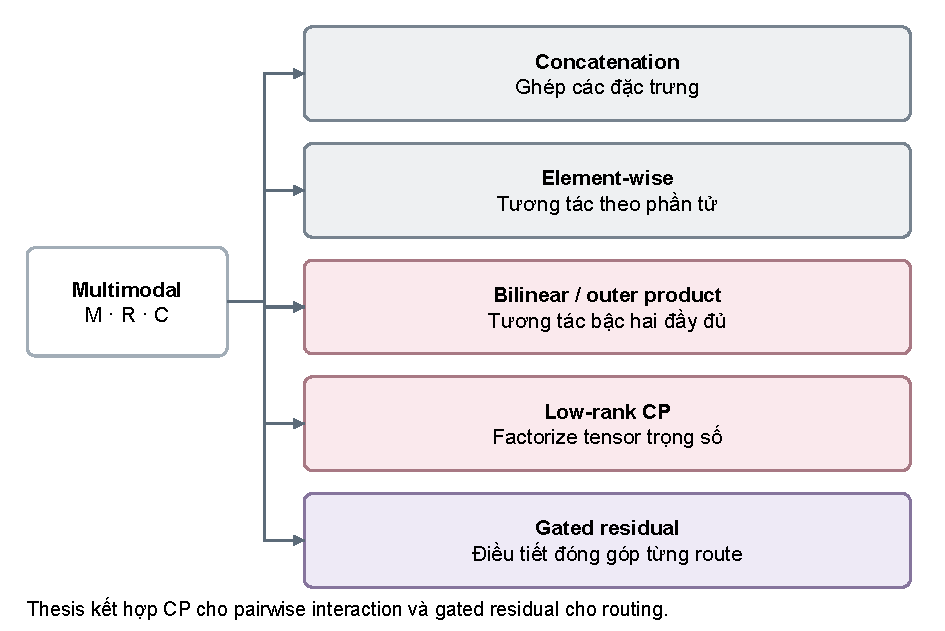
\includegraphics[width=\textwidth]{image/fusion-taxonomy.pdf}
\caption[Phân loại các chiến lược hợp nhất đa phương thức]{Các chiến lược fusion liên quan đến khóa luận. Concatenation là điểm xuất phát; bilinear/outer-product biểu diễn tương tác tường minh; low-rank factorization kiểm soát số tham số; gate và residual điều chỉnh cách bổ sung tương tác vào biểu diễn gốc. CP và gated residual là hai lựa chọn có thể kết hợp trong cùng khối fusion.}
\label{fig:fusion-taxonomy}
\end{figure}

\textbf{Concatenation} nối các vector và để MLP phía sau học quan hệ. \textbf{Tích từng phần tử} tạo tương tác đơn giản sau khi các vector được đưa về kích thước tương thích, nhưng không liệt kê đầy đủ mọi cặp chiều. \textbf{Bilinear/outer-product fusion} mô hình hóa trực tiếp tích chéo giữa các chiều; Tensor Fusion Network là một ví dụ tiêu biểu trong học đa phương thức \cite{zadeh2017tensor}. \textbf{Low-rank fusion} ràng buộc cấu trúc trọng số để giảm độ phức tạp \cite{liu2018lowrank}. \textbf{Adaptive/gated fusion} bổ sung một cơ chế chọn mức đóng góp phụ thuộc đầu vào.

Với cohort nhỏ, biểu diễn phong phú hơn cũng có thể làm tăng phương sai ước lượng. Vì vậy, trình tự của project là thiết lập concatenation, khảo sát pairwise tương tác đầy đủ, rồi mới thay lõi bằng CP và kiểm tra khả năng rút gọn topology. Đây là các giả thuyết thiết kế cần bằng chứng validation, không phải một bảng xếp hạng cố định giữa các loại fusion.

\section{Tương tác song tuyến và phân rã tensor}
Với $x\in\mathbb{R}^{d_x}$ và $y\in\mathbb{R}^{d_y}$, outer-product $xy^{\top}$ chứa mọi tích $x_i y_j$. Flatten ma trận này rồi dùng một lớp linear tương đương ánh xạ song tuyến
\begin{equation}
 h_k=\sum_{i=1}^{d_x}\sum_{j=1}^{d_y}W_{kij}x_i y_j+b_k,
\end{equation}
với tensor trọng số $W\in\mathbb{R}^{d_o\times d_x\times d_y}$. Lõi trọng số chứa $d_od_xd_y$ tham số, chưa tính bias.

CP decomposition biểu diễn tensor như tổng các tensor hạng một \cite{carroll1970candecomp,kolda2009tensor}. Áp dụng cấu trúc này cho \emph{tensor trọng số của lớp song tuyến}, với rank $Q$, cho
\begin{equation}
 W_{kij}\approx\sum_{q=1}^{Q}O_{kq}A_{iq}B_{jq},
 \qquad
 h=O\big[(A^{\top}x)\odot(B^{\top}y)\big]+b.
\end{equation}
Các factor $A$, $B$ và $O$ được học; không cần dựng outer-product tường minh. Lõi trọng số còn $Q(d_x+d_y+d_o)$ tham số. Biểu thức này là cơ sở cho phép thay thế controlled CP của khóa luận; số đếm trong implementation còn tính các bias và được báo cáo riêng ở Chương~\ref{chap:results}.

Low-rank Multimodal Fusion khai thác các factor theo phương thức \cite{liu2018lowrank}, trong khi MUTAN dùng cấu trúc Tucker cho bilinear fusion \cite{benyounes2017mutan}. Các công trình này cung cấp cơ sở về tham số hóa tensor; chúng không chứng minh trực tiếp CP sẽ cải thiện tiên lượng AD. Đặc biệt, trong mô hình của khóa luận, CP factorizes the bilinear interaction weight tensor; dữ liệu MRI/radiomics/lâm sàng của một bệnh nhân không bị phân rã CP trong forward pass.

\section{Gated residual fusion}
Ryumina và cộng sự dùng một phương thức neo, gate phụ thuộc đầu vào và residual hiệu chỉnh trong Text Residual Fusion \cite{ryumina2026residual}. Liu và cộng sự đưa skeleton vào nhánh RGB qua gated residual với hệ số scale cố định $\alpha=0.5$ \cite{liu2026motion}. Đây là hai nghiên cứu ở các tác vụ khác với tiên lượng AD, cung cấp cảm hứng thiết kế về điều tiết đóng góp và scaling.

Lấy cảm hứng từ gated residual modulation trong \cite{ryumina2026residual} và explicit residual scaling trong \cite{liu2026motion}, khóa luận xây dựng cập nhật residual riêng cho từng route:
\begin{equation}
 Z_d=\mathrm{LN}\left[U_d+\sum_{p\in\mathcal{P}(d)}
 \lambda_{p\rightarrow d}\,g_{p\rightarrow d}\,E_{p\rightarrow d}\right].
\label{eq:background-route}
\end{equation}
$U_d$ là biểu diễn gốc của phương thức đích ở không gian residual; $E_{p\rightarrow d}$ là tương tác đã chiếu về cùng không gian; $g_{p\rightarrow d}$ thay đổi theo đầu vào của bệnh nhân--visit; $\lambda_{p\rightarrow d}$ là scalar học được, dùng chung cho route qua các mẫu. Hai bài báo không đề xuất nguyên vẹn công thức này. Khóa luận thích nghi ý tưởng thành định tuyến pairwise theo đích, đồng thời thay scale cố định bằng tham số học theo route.

Identity residual giữ một đường truyền cho thông tin phương thức gốc; gate và scale kiểm soát phần hiệu chỉnh nhưng không tự bảo đảm cải thiện hiệu năng. Layer normalization \cite{ba2016layernorm} được áp dụng sau tổng residual. Dropout \cite{srivastava2014dropout} giúp regularize các MLP; tối ưu dùng AdamW \cite{loshchilov2019adamw}, phát triển từ Adam \cite{kingma2015adam} với weight decay tách khỏi cập nhật gradient. Vai trò thực nghiệm của gate, scale và residual được đánh giá bằng ablation.

\section{Các nghiên cứu liên quan}
Các công trình trong Bảng~\ref{tab:related} có sự khác biệt về cohort, thời điểm dự báo, nhãn và metric. Do đó, bảng dùng để nhận diện lựa chọn phương pháp và khoảng trống, không so sánh trực tiếp số hiệu năng giữa các bài báo với thesis.

\begin{table}[htbp]
\centering
\caption{Các nghiên cứu liên quan và vị trí của khóa luận. Hai công trình cuối có tác vụ khác với survival ranking, nhưng cung cấp góc nhìn về cấu trúc tensor và fusion thích nghi.}
\label{tab:related}
\small
\setlength{\tabcolsep}{4pt}
\begin{tabularx}{\textwidth}{L{3.5cm}L{4.1cm}Y}
\toprule
\textbf{Nghiên cứu} & \textbf{Đầu vào và tác vụ} & \textbf{Liên hệ phương pháp} \\
\midrule
\mbox{Li--Fan (2019)} \cite{li2019early} & MRI hồi hải mã baseline; nhận thức dọc một năm; tiên lượng tiến triển. & Mạng hồi tiếp kết hợp tín hiệu thời gian với MRI. \\
\mbox{Ding (2023)} \cite{ding2023progression} & Biến nhân khẩu, nhận thức và đo đạc ảnh tại năm mốc; chuyển đổi hai năm. & LSTM dọc so với random forest tại index exam. \\
\mbox{Bapat (2024)} \cite{bapat2024fouryear} & MRI 3D và nhận thức dọc; chuyển đổi trong bốn năm. & CNN 3D trích đặc trưng, concatenation rồi CNN 1D. \\
\mbox{Aghajanian (2025)} \cite{aghajanian2025longitudinal} & MRI T1 dọc và radiomics; mô hình sống còn. & CNN--T-LSTM--attention; nguồn baseline trực tiếp của project. \\
\mbox{Zhang (2023)} \cite{zhang2023explainable} & Đặc điểm cấu trúc não dọc; dự báo MMSE/ADAS-Cog. & Tensor multi-task và ensemble; khác CP trọng số pairwise. \\
\mbox{Li (2026)} \cite{li2026longitudinal} & sMRI và clinical dọc; phân loại NC/MCI/AD. & Brain latent diffusion và MoE điều tiết các biểu diễn. \\
\bottomrule
\end{tabularx}
\end{table}

Aghajanian và cộng sự sử dụng 228 người MCI, mỗi người có ba MRI T1 trong 18 tháng; chuỗi CNN embedding được đưa vào T-LSTM có attention. Radiomics không cải thiện nhất quán, và thảo luận của bài báo lưu ý vai trò của huấn luyện hai bước và ensemble \cite{aghajanian2025longitudinal}. Vì vậy, khi chuyển ý tưởng vào project hiện tại, cần phân biệt lợi ích của thông tin dọc với lợi ích của encoder, quy trình huấn luyện và cơ chế fusion.

Zhang và cộng sự dự báo điểm nhận thức bằng tensor multi-task learning và ensemble \cite{zhang2023explainable}; công trình này giúp hình thành ý tưởng dùng cấu trúc tensor trong giai đoạn tìm hiểu. Khóa luận sau đó chuyển trọng tâm sang CP cho \emph{trọng số} tương tác song tuyến trong pipeline sống còn. Li và cộng sự dùng MoE cho phân loại trạng thái chẩn đoán \cite{li2026longitudinal}; cơ chế thích nghi có liên hệ với fusion, nhưng tác vụ này không tương đương với dự báo thời gian tiến triển.

\section{Khoảng trống nghiên cứu}
Khóa luận đặt ba câu hỏi trong cohort và pipeline hiện tại: tương tác tường minh bổ sung gì cho concatenation; CP có giữ hiệu năng hữu ích khi chỉ thay lõi bilinear và giữ các khối khác; và cặp trực tiếp nào cần giữ sau factorization? Chương tiếp theo triển khai kiến trúc và residual routing thích nghi; các so sánh có kiểm soát cùng validation ở Chương~\ref{chap:results} kiểm tra các giả thuyết này.
